\documentclass{school-22.211-notes}
\date{April 25, 2012}

\begin{document}
\maketitle

\lecture{Point Kinetics Without Feedback}
In this section, we would discuss: 
\begin{enumerate}
\item The importance of neutron precursor data ($\beta$) and emission spectram ($\chi$) and how they are being treated in diffusion equation. 

\item Delayed neutron physics. 

\item Delayed neutron models: PKE (know how to solve), prompt jump approximation, In-hour equation, IK. 
\end{enumerate}


\topic{Physics of Delayed Neutrons}
\textbf{Prompt neutrons}: more than 99\% of all neutrons are emitted in $<10^{-10}$s after the fission (prompt neutron lifetime in a PWR is about $2 \times 10^{-5}$ sec). 

\vspace{0.5cm}
\textbf{Delayed neutrons}:
\begin{enumerate}
\item Importance. Assume no delayed neutrons, a reactor was operated at 1W, a control rod was moved to produce an excess reactivity of $0.0005 \Delta k$, what would the power be 1s later? 
\begin{align}
P(t) &= P_0 (1.0005)^{t/(2\times 10^{-5})} = 1 W (1.0005)^{1/(2\times 10^{-5})} = 70,000 MW 
\end{align}
This reactor would be virtually impossible to control! Fortunately, delayed netrons exist and the reactor time constant depend on more than just prompt neutron lifetime. 

\item Review steady-state diffusion equation, and notice: 
  \begin{itemize}
  \item $\chi$ is the spectrum. So integrating $\chi$ over all energy should always give us 1. 
  \item $\chi_d^i (E)$: delayed neutron groups, typically 6-8 groups. 
  \item $\beta^j$ is delayed neutron fraction. 
  \end{itemize}

\item Measurement: delayed neutrons can be measured by counting neutrons emission after a pulsed irradiation of a pure U235 foil. 
  \begin{itemize}
  \item Burst measurement: the amount of prompt neutrons.
  \item Saturated measurement: the total amount of neutrons. 
  \item Measurement vs. evaluation: the data are recorded from measurements, but upon different evaluations the final data would be different. 
  \end{itemize}

\item Neutron Precursor data. Delayed neutrons are emitted through the decay of fission products. 
  \begin{itemize}
  \item Br-87 is a dominant FP that emits delayed neutrons (longest half-life). 
  \item Delayed neutron precursors are embedded in fission species delayed yields. 
    \end{itemize}

\item  \textcolor{blue}{Delayed yields ($\beta$) depend on fissioning species and neutron energy.}
  \begin{itemize}
  \item Absolute yield: number of delayed neutrons per fission; unit: 1/fission. 
  \item Relative yield: absolute yield of an isotope divided by total absolute yield by all isotopes. 
  \item \hi{Delayed neutron fraction $\beta$: absolute yield (\# of delayed neutrons per fission) divided by $\bar{\nu}$ (total fission neutrons) = percentage of neutrons that are delayed.}
  \item 6 group yields and decay constants depend on fissioning species, as in Table~\ref{yield-depend-on-species}.
    \begin{table}[ht]
      \centering
      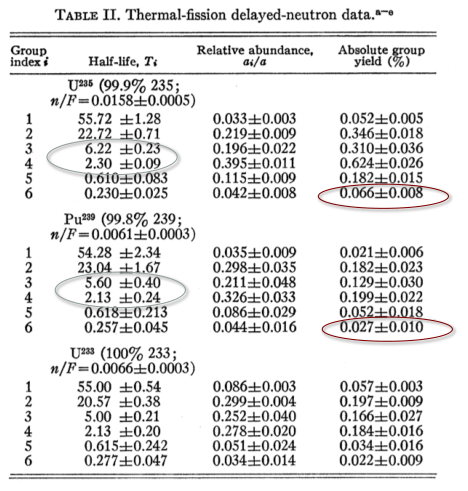
\includegraphics[width=4in]{images/pke/yield-depend-on-species.png}
      \caption{Yields and decay constants depend on fissioning species} \label{yield-depend-on-species}
    \end{table}
  \item \textcolor{blue}{U238 produce 4\% delayed neutron per fission, more than U235's 1.7\% delayed neutron per fission}, making U238 a very important isotope when it comes to delayed neutrons. Fast group absolute yield for U238 is 0.0412, U235 is 0.0165, U239 is 0.0063 as in Table~\ref{abs-yield}. Keep in mind:  model the $\chi$ term technically we need to know the delayed neutron spectrum etc. 
  \end{itemize}
  \begin{table}[ht]
    \centering
    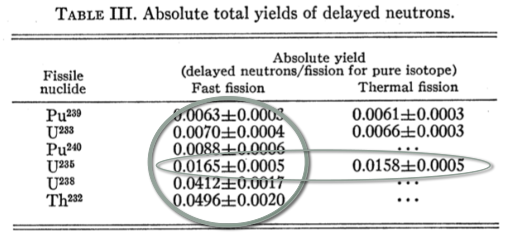
\includegraphics[width=4in]{images/pke/abs-yield.png}
    \caption{Absolute Total Yields of Delayed Neutrons} \label{abs-yield} 
  \end{table}

\item Modeling $\beta$. There are two ideas,  
  \begin{itemize}
  \item Why not use direct measured fission product yields and measured fission product neutron emission rates? Issue: insufficient data to use directly for production analysis. There is a fairly large difference between experimental data and calculated data, making it hard to find a direct agreement on what is the correct fission product yields and emissionrates. 
  \item Keep track of all precursors. We make a 6-group to 8-group model\footnote{Typically 8-group and above would start to produce good fitting; anything less than 8 group you run into the risk of having too many precursors/half-lives lumped in the same energy group and causing trouble.}, and each group has a fixed/homogeneous decay constants (the one that dominants in the group, that is, largest half-life). This way, all isotopes have the same half-life for the same group; but different isotopes would still have different delayed neutron fraction. Remember the terms circled in blue in Table~\ref{8-group-data} (the delayed neutron fraction listed in this table might be in \% unit, because U235 thermal fission fraction should be 0.0067.).  
    \begin{table}[ht]
      \centering
      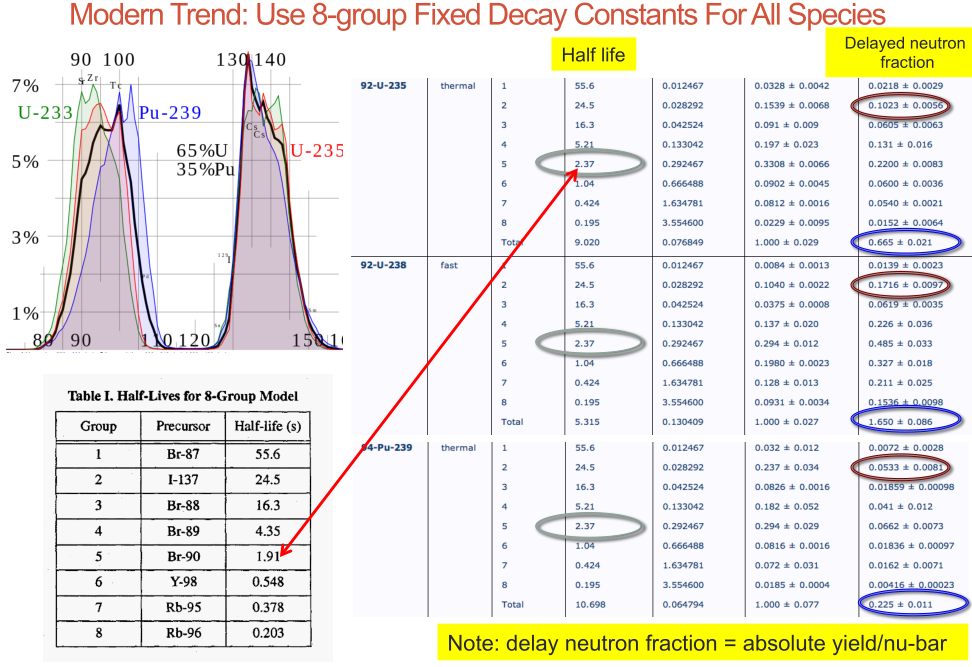
\includegraphics[width=7in]{images/pke/8-group-fixed-decay-constants.png}
      \caption{8-group Fixed Decay Constans for All Species} \label{8-group-data}
    \end{table}
  \end{itemize}


\item Delayed neutrons spectrum $\chi$.
  \begin{itemize}
  \item U238 is extremely important for delayed neutrons.
  \item Delayed neutrons are produced at lower energy than prompt neutrons: average prompt neutron emission energy is 2 MeV; average delayed neutron emission energy is 0.4 MeV. 
  \item Delayed neutron comes out in the thermal energy range, which makes them more likely to fission. 
  \item Both spectrum comes out to be Maxwellian shapes for all the delayed groups, except the delayed one is shifted as in Fig.~\ref{fission-spec}. Keep in mind that these Maxwellian curves we use are approximations; real data is often discrete in nature. 
    \begin{figure}[ht]
      \centering
      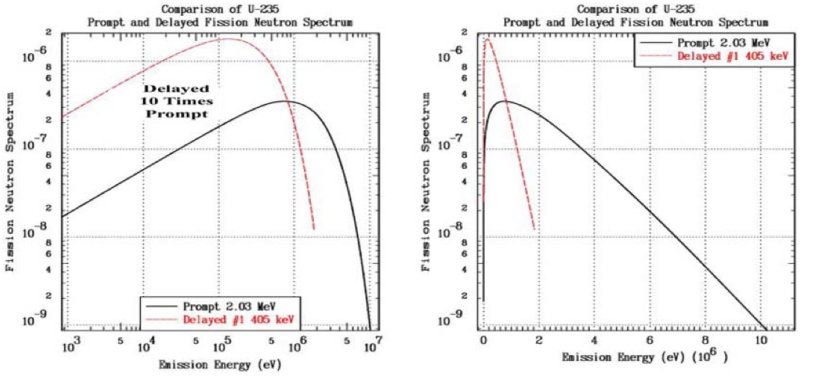
\includegraphics[width=4in]{images/pke/fission-spec.png}
      \caption{Prompt and Delayed Fission Neutron Spectrum} \label{fission-spec}
    \end{figure}
  \item Delayed energy group: neutron spectra have similar shapes for all delayed groups. However different energy groups have different mean energies. 
    \begin{figure}[ht]
      \centering
      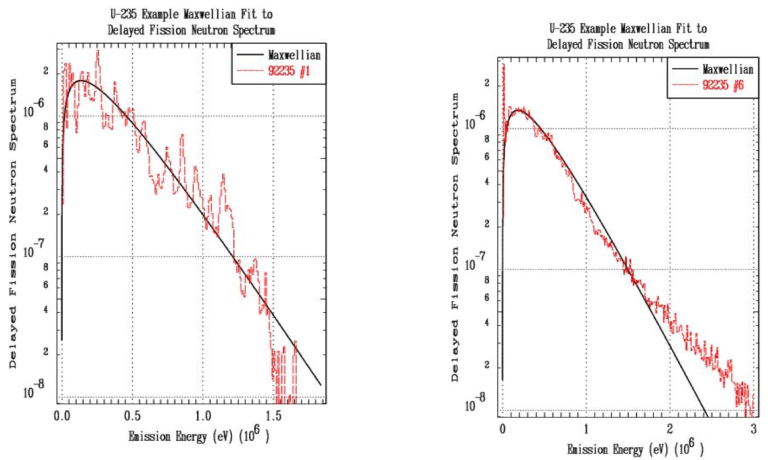
\includegraphics[width=4in]{images/pke/delayed-fission-spec.png}
      \caption{Delayed Fission Neutron Spectrum} \label{delayed-fission-spec} 
    \end{figure}
  \item Summary: \hi{Delayed neutron spectra vary only slightly for different fissioning nuclides; but the spectra depends significantly on the delayed neutron group} (in real production tools, there is a separate $\chi$ for each energy group). 
  \end{itemize}
\end{enumerate}

\clearpage
\topic{Derivation of PKE from Diffusion Equation}
\begin{enumerate}
\item We start from the diffusion equation: \hi{The steady-state diffusion equation}\footnote{Know this for the final}: 
\small
\begin{align}
& - \divergence D(\vecr, E) \gradient \phi(\vecr, E) + \Sigma_t (\vecr, E) \phi(\vecr, E) = \int_0^{\infty} \Sigma_s (\vecr, E'\to E) \phi(\vecr, E') \dE' \\
&+ \Sum_j \chi_T^j (E) \int_0^{\infty} \nu \Sigma_p^j (\vecr, E') \phi(\vecr, E') \dE' + Q(\vecr, E) 
\end{align}
\normalsize
\begin{itemize}
\item In steady-state transport or diffusion equation, we do not treat delayed neutrons directly. Instead the fission emission spectrum must be properly weighted with prompt and delayed contributions. 

\item A chicken-and-egg problem: we need fission rates to compute $\chi(E)$, and we need $\chi(E)$ to get fission rates, so the real way to solve the balance equation is to iterate, though this is not how it is done normally.
\end{itemize}


\item \hi{The time-dependent neutron diffusion equation}: in transient diffusion equations, the delayed neutrons must be treated explicitly. $\beta^j = \Sum_i \beta_i^j$ is the delayed fission fraction (0.66\% for instance), 
  \begin{align}
    \ppt \left[ \frac{1}{v} \phi(\vecr, E, t) \right] &= \divergence D(\vecr, E, t) \gradient \phi(\vecr, E, t) - \Sigma_t (\vecr, E, t) \phi(\vecr, E, t) 
\notag \\
    & + \int_0^{\infty} \Sigma_s (\vecr, E'\to E, t) \phi(\vecr, E', t) \dE'\notag \\
    &+ \Sum_j \chi_p^j (E) (1-\beta^j) \int_0^{\infty} \nu \Sigma_f^j (\vecr, E', t) \phi(\vecr, E', t) \dE'\notag \\
    &+ \Sum_i \chi_d^i (E) \lambda_i C_i (\vecr, t) + Q(\vecr, E, t)\\
    \ppt C_i (\vecr, t) &= \Sum_j \beta_i^j \int_0^{\infty} \nu \Sigma_p^j (\vecr, E', t) \phi(\vecr, E', t) \dE'  - \lambda_i C_i (\vecr, t) 
  \end{align}
  where $i$ is for isotropes, $j$ is for energy groups. 

\item Assume that flux can be separated into a space/energy term and a time-dependent term: 
  \eqn{ \phi(\vecr, E, t) = S(\vecr, E) T(t) }
where $S(\vecr, E)$ is the Shape function,  $T(t)$ is the amplitude function (remember this approximation may not always be valid, and certainly in some cases it would not be a good approximation). Plug it into the above expressions. 
  \begin{align}
    \ppt \left[ \frac{1}{v} S(\vecr, E) T(t) \right] &= 
    \Bigg\{ \divergence D(\vecr, E, t) \gradient S(\vecr, E) - \Sigma_t (\vecr, E, t) S(\vecr, E)   \notag \\
    & + \int_0^{\infty} \Sigma_s (\vecr, E'\to E, t) S(\vecr, E') \dE'   \notag \\
    &+ \Sum_j \left( \chi_p^j (E) (1-\beta^j) + \Sum_i \chi_d^i (E) \beta_i^j \right) \int_0^{\infty} \nu \Sigma_f^j (\vecr, E', t) S(\vecr, E') \dE'   \notag \\
    &- \Sum_j \chi_p^j (E) \beta^j \int_0^{\infty} \nu \Sigma_f^j (\vecr, E', t) S(\vecr, E') \dE' \Bigg\} T(t)  \notag \\
    &+ \Sum_i \chi_d^i (E) \lambda_i C_i (\vecr, t) + Q(\vecr, E, t)   \\
    \ppt C_i (\vecr, t) &= \left\{ \Sum_j \beta_i^j \int_0^{\infty} \nu \Sigma_p^j (\vecr, E', t) S(\vecr, E') \dE' \right\} T(t) - \lambda_i C_i (\vecr, t) 
  \end{align}


\item Integrate over all space and energy and normalize to $\int \dE \int \dr \frac{1}{v} S(\vecr, E) = 1.0$, 
  \begin{align}
    \ddt \left[ T(t) \right] &= 
    \int \dE \int \dr \Bigg\{ \divergence D(\vecr, E, t) \gradient S(\vecr, E) - \Sigma_t (\vecr, E, t) S(\vecr, E)   \notag \\
    & + \int_0^{\infty} \Sigma_s (\vecr, E'\to E, t) S(\vecr, E') \dE'   \notag \\
    &+ \Sum_j \left( \chi_p^j (E) (1-\beta^j) + \Sum_i \chi_d^i (E) \beta_i^j \right) \int_0^{\infty} \nu \Sigma_f^j (\vecr, E', t) S(\vecr, E') \dE'   \notag \\
    &- \Sum_j \chi_p^j (E) \beta^j \int_0^{\infty} \nu \Sigma_f^j (\vecr, E', t) S(\vecr, E') \dE' \Bigg\} T(t)  \notag \\
    &+ \int \dE \int \dr \left[ \Sum_i \chi_d^i (E) \lambda_i C_i (\vecr, t) + Q(\vecr, E, t)\right]   \label{PKE-1}
  \end{align}
  \begin{align}
    \ddt \left[ \int \dE \int \dr C_i (\vecr, t) \right] &= \int \dE \int \dr \left\{ \Sum_j \beta_i^j \int_0^{\infty} \nu \Sigma_p^j (\vecr, E', t) S(\vecr, E') \dE' \right\} T(t) \notag \\
    &- \lambda_i \int \dE \int \dr C_i (\vecr, t)  \label{PKE-2}
  \end{align}


\item Simplify energy dependency. In Eq.~\ref{PKE-1}, notice in the term $\Sum_j \chi_p^j (E) \beta^j \int_0^{\infty} \nu \Sigma_f^j (\vecr, E', t) S(\vecr, E') \dE'$, only $\chi_p^j(E)$ depends on energy, we can use $\int \chi_p^j (E) \dE = 1$ to get rid of the energy integral in Eq.~\ref{PKE-1}, 
  \begin{align}
    \ddt \left[ T(t) \right] &= 
    \int \dE \int \dr \Bigg\{ \divergence D(\vecr, E, t) \gradient S(\vecr, E) - \Sigma_t (\vecr, E, t) S(\vecr, E)   \notag \\
    & + \int_0^{\infty} \Sigma_s (\vecr, E'\to E, t) S(\vecr, E') \dE'   \notag \\
    &+ \Sum_j \left( \chi_p^j (E) (1-\beta^j) + \Sum_i \chi_d^i (E) \beta_i^j \right) \int_0^{\infty} \nu \Sigma_f^j (\vecr, E', t) S(\vecr, E') \dE'  \Bigg\} T(t)  \notag \\
    &- \int \dr \Bigg\{ \Sum_j \beta^j \int_0^{\infty} \nu \Sigma_f^j (\vecr, E', t) S(\vecr, E') \dE' \Bigg\} T(t)  \notag \\
    &+ \int \dE \int \dr \left[ \Sum_i \chi_d^i (E) \lambda_i C_i (\vecr, t) + Q(\vecr, E, t)\right]   \label{PKE-3}
  \end{align}
  In a similar fashion, notice Eq.~\ref{PKE-2} no term has a $E$ dependency, so we can cross out the $\int \dE$ in every term to get, 
    \begin{align}
    \ddt \left[ \int \dr C_i (\vecr, t) \right] &= \int \dr \left\{ \Sum_j \beta_i^j \int_0^{\infty} \nu \Sigma_p^j (\vecr, E', t) S(\vecr, E') \dE' \right\} T(t) \notag \\
    &- \lambda_i \int \dr C_i (\vecr, t)  \label{PKE-4}
  \end{align}


\item Assume no net current (leakage) out of the reactor model\footnote{Recall we used Gauss theory to make the volume integral into surface integral, thus creating zero leakage for certain BCs.}, thus $\divergence D(\vecr, E, t) \gradient S(\vecr, E) \to 0$. Assume no external source of prompt or delayed neutrons, thus $Q(\vecr, E, t) \to 0$. 


\item Assume \hi{prompt fission spectrum $\chi_d^j$ is independent of fissioning species $j$}, that is, we drop the $j$ dependency on prompt terms $\chi_p^j, \beta^j$, 
\eqn{ \Sum_j \chi_p^j (1 - \beta^j) = \chi_p (1 - \beta) }

\item Assume \hi{delayed fission yield $\beta^j$ is independent of fissioning species $j$}, that is, we drop the $j$ dependency on delayed terms, 
\eqn{ \Sum_j \beta^j &= \beta  & \Sum_j \beta_i^j &= \beta_i }
The last two assumptions together, we can write $\Sigma_f^j \to \Sigma_f$. 

\item Assume \hi{delayed fission spectrum $\chi_d^i$ is independent of delayed neutron group $i$}\footnote{we saw from data two lectures ago that $\chi$ is slightly dependent on neutron group, but we don't care much about it for this context.}, that is, we drop the $i$ dependency on $\chi_d^i$, 
\eqn{ \Sum_i \chi_d^i (E) \lambda_i C_i = \chi_d (E) \Sum_i \lambda_i C_i }

\item Assume \hi{delayed neutron yield $\beta$ is independent of space}, together with the last assumption, we can write, 
\eqn{ \Sum_j \Sum_i \chi_d^i (E) \beta_i^j  = \chi_d (E) \beta }
Thus we reach, 

  \begin{align}
    \ddt \left[ T(t) \right] &= 
    \int \dE \int \dr \Bigg\{  - \Sigma_t (\vecr, E, t) S(\vecr, E)   + \int_0^{\infty} \Sigma_s (\vecr, E'\to E, t) S(\vecr, E') \dE'   \notag \\
    &+ \left\{ \chi_p (E) (1-\beta) + \chi_d (E) \beta \right\} \int_0^{\infty} \nu \Sigma_f^j (\vecr, E', t) S(\vecr, E') \dE'  \Bigg\} T(t)  \notag \\
    &-  \beta \int \dr \Bigg\{ \int_0^{\infty} \nu \Sigma_f (\vecr, E', t) S(\vecr, E') \dE' \Bigg\} T(t)  
    + \int \dE \int \dr \left[ \chi_d (E) \Sum_i \lambda_i C_i (\vecr, t) \right]   \label{PKE-5}
  \end{align}
    \begin{align}
    \Aboxed{ \ddt \left[ \int \dr C_i (\vecr, t) \right] &=  \beta_i \int \dr \left\{ \int_0^{\infty} \nu \Sigma_f (\vecr, E', t) S(\vecr, E') \dE' \right\} T(t)  - \lambda_i \int \dr C_i (\vecr, t)  } \label{PKE-6}
  \end{align}


\item We further assume that $\int \dE \chi_d (E)  = 1$, thus the last term simplifies, and two long terms cancel out, 
  \eqn{ \int \dE \dr \chi_d(E) \beta \int_0^{\infty} \nu \Sigma_f^i (\vecr, E', t) S(\vecr, E') \dE' T(t) - \beta \int \dr \int_0^{\infty} \nu \Sigma_f (\vecr, E' t) S(\vecr, E') \dE' T(t) = 0  \notag } 
Thus Eq.~\ref{PKE-5} becomes, 
  \begin{align}
    \ddt \left[ T(t) \right] &= 
    \int \dE \int \dr \Bigg\{  - \Sigma_t (\vecr, E, t) S(\vecr, E)   + \int_0^{\infty} \Sigma_s (\vecr, E'\to E, t) S(\vecr, E') \dE'   \notag \\
    &+ \chi_p (E) (1-\beta) \int_0^{\infty} \nu \Sigma_f (\vecr, E', t) S(\vecr, E') \dE'  \Bigg\} T(t)  +  \int \dr  \Sum_i \lambda_i C_i (\vecr, t)    \label{PKE-7}
  \end{align}


\item Traditionally we weight the PKEs by adjoint flux, not by unity.  We add $\phi^*$ because the prompt neutron spectrum has energy dependency, but no $\phi^*$ for precursors because precursors emission is not energy dependency, it is just a fission rate.\footnote{We add $\int \dE$ back on the last term in Eq.~\ref{PKE-7} after adding in $\phi^*$. We give $\beta_i$ its spatial dependency back in both equations. Though $\lambda_i$ does not depend on fissioning species, meaning they are not spatially dependence.}
  \begin{align}
  \Aboxed{ \ddt \left[ T(t) \right] &=  
    \int \dE \int \dr  \phi^* (\vecr, E) \left\{  - \Sigma_t (\vecr, E, t) S(\vecr, E)   + \int_0^{\infty} \Sigma_s (\vecr, E'\to E, t) S(\vecr, E') \dE'  \right. } \notag \\
    \Aboxed{ &+  \left. \chi_p (E) (1-\beta (\vecr)) \int_0^{\infty} \nu \Sigma_f (\vecr, E', t) S(\vecr, E') \dE'  \right\} T(t)  + \int \dE \int \dr \phi^*(\vecr, E)  \chi_d (E) \Sum_i \lambda_i C_i (\vecr, t)  }   \label{PKE-8}
  \end{align}
\end{enumerate}



\topic{Multi-Group PKEs}
Based on Eq.~\ref{PKE-6} and Eq.~\ref{PKE-8}, 
\begin{enumerate}
\item \hi{Multi-group PKEs}: normalize $\Sum_g \expect{ \int \dr \phi_g^* (\vecr) \frac{1}{v_g(\vecr, t)} S_g (\vecr) } = 1.0$, we basically add a $_g$ subscript to every term applicable, and convert any $\int \dE A(E)$ to $\Sum_{g} A_{g}$, 
  \begin{align}
 \ddt \left[ T(t) \right] &=  
    \int \dr  \phi_g^* (\vecr)  \left\{  - \Sigma_{t,g} (\vecr, t) S_g(\vecr) T_g(t)   + \Sum_{g'} \Sigma_{s, g' \to g} (\vecr, t) S_{g'}(\vecr) T_{g'} (t)  \right.  \notag \\
    &+  \left. \chi_{p,g} (E) (1-\beta (\vecr)) \Sum_{g'} \nu \Sigma_{f,g'} (\vecr, t) S_{g'} (\vecr) T_{g'}(t) \right\}  + \int \dr \phi^*(\vecr) \chi_{d,g}  \Sum_i \lambda_i C_i (\vecr, t)    \label{PKE-9}  \\
     \ddt \left[ \int \dr C_i (\vecr, t) \right] &=   \int \dr \beta_i (\vecr) \Sum_g \nu \Sigma_{f,g} (\vecr, t) S_g (\vecr) T_g(t)   - \lambda_i \int \dr C_i (\vecr, t)  \label{PKE-10}
  \end{align}


\item \hi{2-group PKEs}\footnote{Very Important! Know this for the exam!!!}:
  \begin{align}
  \ddt \left[ T_1(t) \right] &=   \int \dr  \phi_1^* (\vecr)  \left\{  - \Sigma_{r,1} (\vecr,t) S_1(\vecr) T_1(t)  + [1-\beta (\vecr)][\nu \Sigma_{f,1} (\vecr, t) S_{1} (\vecr) T_{1}(t) + \nu \Sigma_{f,2} (\vecr, t) S_2 (\vecr) T_2 (t)] \right\} \notag \\
    &+ \int \dr \phi^*(\vecr)   \Sum_i \lambda_i C_i (\vecr, t)     \label{PKE-11} \\
   \ddt \left[ T_2(t) \right] &=  
    \int \dr  \phi_2^* (\vecr)  \left[ - \Sigma_{a,2} (\vecr,t) S_2(\vecr) T_2(t) + \Sigma_{s12} (\vecr, t) S_1 (\vecr) T_1 (t)  \right]   \label{PKE-12}
  \end{align}
  \begin{align}
   \ddt \left[ \int \dr C_i (\vecr, t) \right] &=   \int \dr \beta_i (\vecr) \left[ \nu \Sigma_{f,1} (\vecr, t) S_1 (\vecr) T_1(t) + \nu \Sigma_{f,2} (\vecr, t) S_2 (\vecr) T_2 (t) \right]   - \lambda_i \int \dr C_i (\vecr, t)  \label{PKE-13}
  \end{align}
  The assumptions made include, 
  \begin{enumerate}
    \item No leakage out of the core. 
    \item All fission neutrons born in the fast group. 
    \item All delayed neutron born in the fast group. 
    \item Downscattering is replaced by effective downscattering. No upscattering. 
  \end{enumerate}

\item We can further write the 2-group PKEs in matrix form as in Table~\ref{matrix-2-group-PKEs}. 
  \begin{table}[ht]
    \centering
    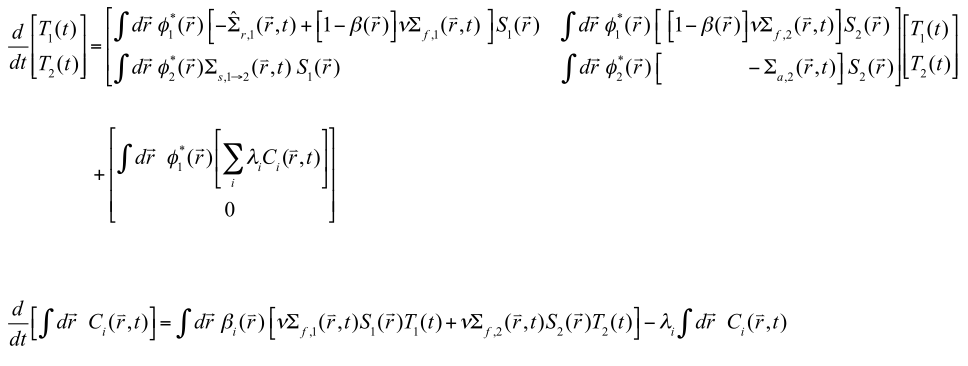
\includegraphics[width=6.5in]{images/pke/matrix-2-group-PKEs.png}
    \caption{Matrix Form of 2-Group PKE Diffusion Equations} \label{matrix-2-group-PKEs}
  \end{table}
\end{enumerate}










\topic{PKE Parameters}
\begin{enumerate}
\item We define a set of terms to simplify the expression. For simplicity concern, we omit the dependency on the following terms. $D(\vecr, E, t), \Sigma_t (\vecr, E, t), \Sigma_f(\vecr, E, t),  S(\vecr, E), \chi(E)$. 
\begin{enumerate}
\item Reactivity $\rho(t)$, where the top is the diffusion equation, and the bottom is fission rate if all the neutrons show up instatenously. 
\eqn{ \rho = \frac{\mbox{net production}}{\mbox{perturbation denomenator (sum of all fission in the system)}} }
\scriptsize
\begin{align}
\rho (t) &= \frac{\int \bsp \dE \! \int \bsp \dr \Bigg\{ \!\divergence \! D  \gradient S  - \! \Sigma_t S  + \! \int \bsp \Sigma_s (\vecr \!, E' \bsp \to \bsp E, t) S \! \dE'   
    + \! \Sum_j \left( \! \chi_p^j (E) (1 \! - \! \beta^j) +  \! \Sum_i \chi_d^i (E) \beta_i^j \! \right) \! \int \bsp \nu \Sigma_f^j  S \dE'  }{\int \bsp \dE \int \bsp \dr \Sum_j \left( \chi_p^j (E) (1-\beta^j) + \Sum_i \chi_d^i (E) \beta_i^j \right) \int \bsp \nu \Sigma_f^j S \dE'} 
\end{align}
\normalsize
\eqn{ \Aboxed{ \rho(t) &= \frac{\keff - 1.0}{\keff}  } }


\item The delayed neutron fraction (notice although this is called delayed neutron fraction, there is $\chi_p^j(E)$ term in it), 
\begin{align}
\beta_i (t) &= \frac{\int \bsp \dE \int \bsp \dr \left[ \Sum_j \chi_d^j (E) \beta^j \int_0^{\infty} \nu \Sigma_f^j (\vecr, E', t) S(\vecr, E') \dE' \right] }{\int \bsp \dE \int \bsp \dr \Sum_j \left( \chi_p^j (E) (1-\beta^j) + \Sum_i \chi_d^i (E) \beta_i^j \right) \int \bsp \nu \Sigma_f^j S \dE'} 
\end{align}
If we don't worry about the fissioning spectra, we would have $\beta \approx \beta_i$. 


\item Prompt neutron lifetime, 
\begin{align}
\Lambda (t) &= \frac{\int \bsp \dE \int \bsp  \dr \left[ \frac{1}{v} S(\vecr, E) \right] }{\int \bsp \dE \int \bsp \dr \Sum_j \left( \chi_p^j (E) (1-\beta^j) + \Sum_i \chi_d^i (E) \beta_i^j \right) \int \bsp \nu \Sigma_f^j S \dE'} 
\end{align}
\eqn{ \Aboxed{ \Lambda(t) &\approx \frac{1}{v \nu \Sigma_f} \xrightarrow{\mathrm{criticality}} \frac{1}{v \Sigma_a} } }
The prompt neutron life $\Gamma \sim 1/v$ of shape divided by almost-instantenous-fission-rate. 
\item The $i$-th precursor, 
  \eqn{ C_i (t) = \int \dE \int \dr C_i (\vecr, t) }
\item The total eternal source, 
  \eqn{ Q(t) = \int \dE \int \dr Q (\vecr, t) }
\end{enumerate}

\item 2-group PKE parameters.  Recall that $\rho(t)$ does not describe how much neutrons there are at a specific time; it describes how much neutrons there would be eventually.  Notice $\beta$ only depends on group 1 because all delayed neutrons are born in group 1. Similarly $\Gamma$ is the prompt neutron life time, thus not depends on $\phi_2^*$ at all. 
\scriptsize
\begin{align}
\rho(t) &= \frac{  \int \dr  \phi_1^* (\vecr)  \left\{  - \Sigma_{r,1} (\vecr,t) S_1(\vecr) T_1(t)  + [\nu \Sigma_{f,1} (\vecr, t) S_{1} (\vecr) T_{1}(t) + \nu \Sigma_{f,2} (\vecr, t) S_2 (\vecr) T_2 (t)] \right\}
+  \int \dr  \phi_2^* (\vecr)  \left[ - \Sigma_{a,2} (\vecr,t) S_2(\vecr) T_2(t) + \Sigma_{s12} (\vecr, t) S_1 (\vecr) T_1 (t)  \right]  }
{\int \dr \phi_1^* (\vecr)  [\nu \Sigma_{f,1} (\vecr, t) S_{1} (\vecr) T_{1}(t) + \nu \Sigma_{f,2} (\vecr, t) S_2 (\vecr) T_2 (t)] } 
\end{align}
\normalsize
\eqn{ \beta_i (t) = \frac{\int \dr \phi_1^* (\vecr) \beta_i (\vecr, t)  [\nu \Sigma_{f,1} (\vecr, t) S_{1} (\vecr)  + \nu \Sigma_{f,2} (\vecr, t) S_2 (\vecr) ] }{\int \dr \phi_1^* (\vecr, t)   [\nu \Sigma_{f,1} (\vecr, t) S_{1} (\vecr) + \nu \Sigma_{f,2} (\vecr, t) S_2 (\vecr) ] } }
\eqn{ \Lambda(t) = \frac{1}{\int \dr \phi_1^* (\vecr, t) [\nu \Sigma_{f,1} (\vecr, t) S_{1} (\vecr) + \nu \Sigma_{f,2} (\vecr, t) S_2 (\vecr) ]} }
\eqn{ C_i (t) = \int \dr C_i (\vecr, t) }

\item Using the defined PKE parameters, we get the classic \hi{point kinetics equations (PKE)},
\eqn{ \Aboxed{ \ddt T(t) &= \frac{\rho(t) - \Sum_i \beta_i (t) }{\Lambda (t)} T(t) + \Sum_i \lambda_i C_i (t) + Q(t) } }
\eqn{ \Aboxed{ \ddt C_i (t) &= \frac{\beta_i (t)}{\Lambda (t)} T(t) - \lambda_i C_i (t) }  }
Remember that the above classic PKEs are obtained using \uline{assumptions}: 
\begin{itemize}
\item No external source.
\item Constant $\beta_i, \lambda_i$. 
\item The approximation $\phi(\vecr, E, t) = S(\vecr, E) T(t)$, which is not always valid. 
\item There is no feedback (e.g., the reactor is operating at low enough flux, no feedback, coefficients are independent of solution), if $\rho(t)$ is known, one can solve for reactor power as a function of time.
\end{itemize}

\item For a steady state solution at power level $T_0$, we know, 
  \begin{align}
    \ddt C_i (0) &= 0  &\Rightarrow  C_i (0) &= \frac{\beta_i}{\Lambda \lambda_i} T_0  \notag \\
    \ddt T(0) &= 0  &\Rightarrow \rho(0) &= 0  \label{in-hour}
  \end{align}

\item \hi{The matrix form of the 1st order ODE} is (assuming three precursor groups, can be easily extend for more precursor groups),  
\begin{align}
N &= \left[ \begin{array}{c} T \\ C_1 \\ C_2 \\ C_3 \end{array} \right]  
& \ddt N(t) &= \left[ \begin{array}{cccc} 
\frac{\rho(t) - \beta}{\Lambda} & \lambda_1 & \lambda_2 & \lambda_3 \\
\frac{\beta_1}{\Lambda} & - \lambda_1 & & \\
\frac{\beta_2}{\Lambda} & & -\lambda_2 & \\
\frac{\beta_3}{\Lambda} & & & -\lambda_3 \end{array} \right] 
\left[ N(t) \right] 
\end{align}
\end{enumerate}

\clearpage
\topic{Application of PKEs}
\begin{enumerate}
\item Instantaneous reactor scram from criticality($\rho = - 8 \beta$). Power goes almost instantly to about 10\%, then it ultimately decays with time constant of longest lived precursor (Br87 with a half-life of 55s). 
  \begin{figure}[ht]
    \centering
    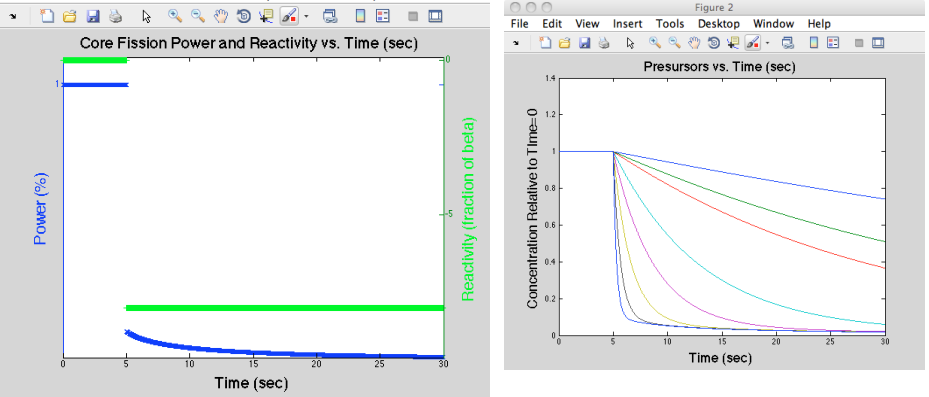
\includegraphics[width=5in]{images/pke/ex1.png}
    \caption{PKE Example 1, Instant Reactor Scram} 
  \end{figure}

\item 2s rod drop scram ($\rho = - 8 \beta$). This is a common assumption to make for real application because rods are dropping to replace the water. Again, power goes to about 10\% when rod fully inserted, and power ultimately decays with time constant of the longest lived precursor (55s).  
  \begin{figure}[ht]
    \centering
    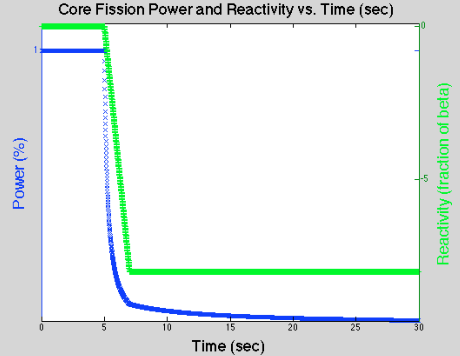
\includegraphics[width=3in]{images/pke/ex2.png}
    \caption{PKE Example 2, Two Second Reactor Scram} 
  \end{figure}

\clearpage
\item Instantaneous rod withdraw ($\rho = 0.1 \beta$). In this senario, there is only one delayed neutron precursor group, and we withdraw rod instantly. \textcolor{blue}{The reactor wants to response immediately (hence the jump) but it does not have enough delayed neutron to sustain that increase, hence the jump is not enough and it will increase for the rest of the way}, until ultimately power increases with time constant of the longest precursor group (55s). See next section for the derivation of prompt jump estimation. 
  \begin{figure}[ht]
    \centering
    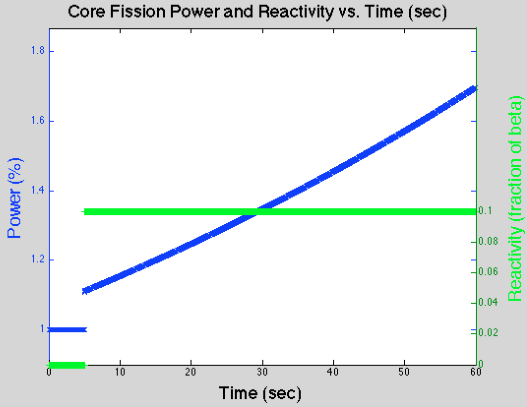
\includegraphics[width=3.5in]{images/pke/ex3.png}
    \caption{PKE Example 3, Instant Rod Withdrawal}  \label{ex3}
  \end{figure}
 


\item \uline{Instantaneous rod withdraw with 8 delayed groups.} The intial part of the transient is slightly more complicated in Fig.~\ref{4a} than 1-group case in Fig.~\ref{ex3}(single delayed group is very sensitive to the time-constant). 

Fig.~\ref{4b} shows that, if we wait long enough, the power becomes an asymptotic exponential rise. We reach \hi{secular equilibrium} between power and precursor rate that the precursor rates have the same shapes as the power, altough the rates may be off by a factor. 
  \begin{figure}[ht]
    \begin{subfigure}[b]{0.45\textwidth}
      \centering
      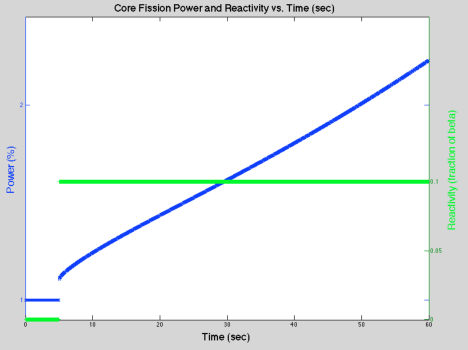
\includegraphics[width=\textwidth]{images/pke/ex4.png}
      \caption{Short Term Behavior} \label{4a} 
    \end{subfigure}
    \begin{subfigure}[b]{0.45\textwidth}
      \centering
      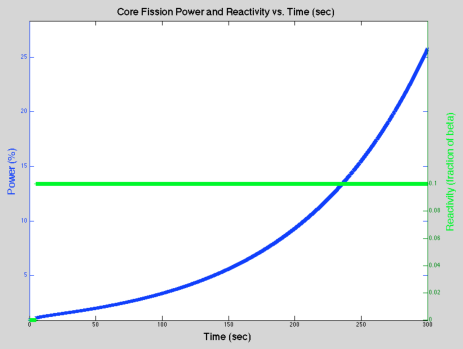
\includegraphics[width=\textwidth]{images/pke/ex4b.png}
      \caption{Long Term Behavior} \label{4b} 
    \end{subfigure}
    \caption{PKE Example 4, Instant Rod Withdrawal With 8 Delayed Groups} \label{ex4}
  \end{figure}

\item \uline{2s rod insertion with 8 delayed groups ($\rho = -0.1 \beta$).}
  \begin{figure}[ht]
    \centering
    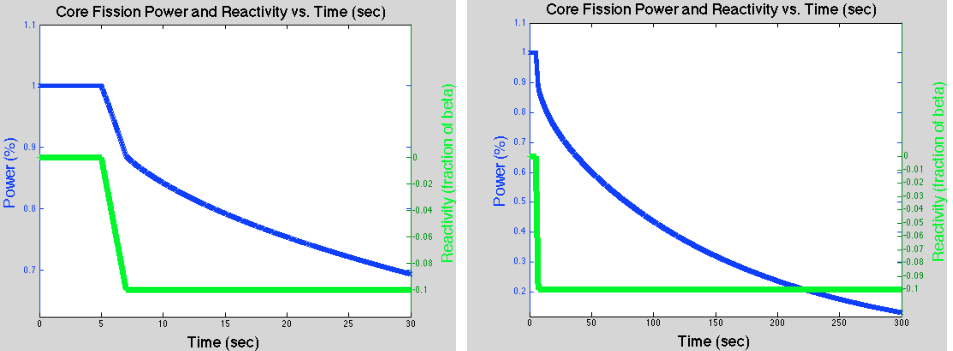
\includegraphics[width=6in]{images/pke/ex5.png}
    \caption{PKE Example 5, Two Second Rod Insertion} 
  \end{figure}

\item \uline{Regulating rod withdrawal/insertion.} Senario: rod is moved in for 2s, hold for 20s, re-positioned in 2s. \textbf{Power does not come back to the original state, because we are solving for an eigenvalue problem, and what the asymptotic power is depends on how to get there.} In the withdrawal case, the precursor builds up and is continuing to build up during the second phase, so the power ends up higher than initially\footnote{it is almost like driving, except there is no friction.}.
  \begin{figure}[ht]
    \centering
    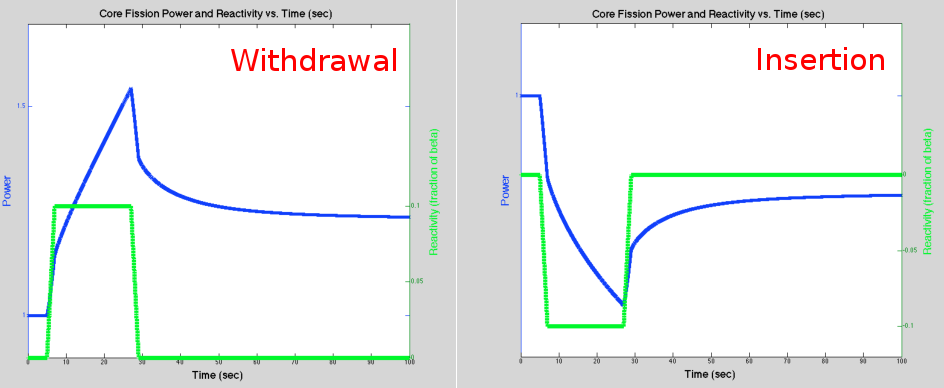
\includegraphics[width=6in]{images/pke/ex6.png}
    \caption{PKE Example 6, Rod Withdrawal and Insertion} 
  \end{figure}

\item \uline{Super-prompt criticality/rod ejection/failed housing.} Senario: rod is moved in for 1s. The point is, power ascension is very sensitive as $\rho \approx \beta$. \textbf{When $\rho > \beta$, reactivity does not have to wait for the delayed neutrons anymore, changes can happen instantaneously.} Thus if your data is more than 5\% uncertain, the answer would vary quite a lot. 
  \begin{figure}[ht]
    \centering
    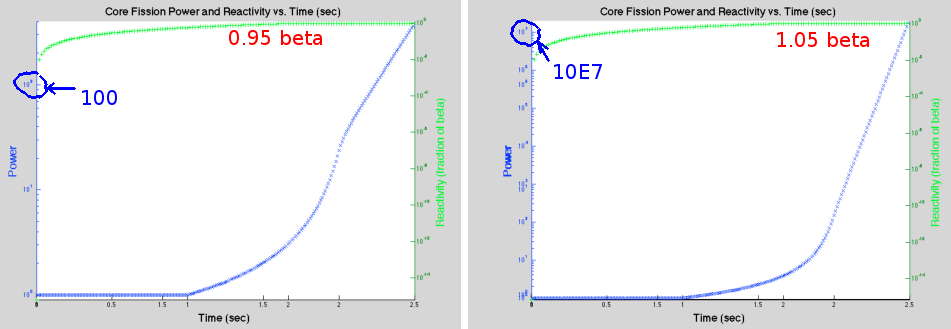
\includegraphics[width=6in]{images/pke/ex7.png}
    \caption{PKE Example 7, Failed Housing} 
  \end{figure}
  
\end{enumerate}



\clearpage
\topic{Prompt-Jump Approximations}
Prompt-jump approximation is used to estimate prompt-jump (of course). 
\begin{enumerate}
\item In a subcritical transient, assume precursors dominant, and prompt neutron changes are negligible, 
\begin{align}
\ddt P(t) &= \frac{\rho - \beta}{\Lambda} P(t) + \Sum_1^K \lambda_k C_k(t) + S (t) \\
\ddt C_k(t) &= \frac{\beta_k}{\Lambda} P(t) - \lambda_k C_k(t) 
\end{align}
We set $\ddt P(t) = 0$, and can solve for $P(t)$ and get an expression for $\ddt C_k(t)$: 
\begin{align}
P(t) &= \frac{\Lambda}{\beta -\rho} S(t) + \frac{\Gamma}{\beta -\rho} \Sum_1^K \lambda_k C_k (t) \\
\ddt C_k (t) &= \frac{\beta_k}{\beta - \rho} S(t) + \frac{\beta_k}{\beta - \rho} \Sum_{k'=1}^K \lambda_{k'} C_{k'} (t) - \lambda_k C_k (t)
\end{align}


\item Assume one precursor group and no source, 
\begin{align}
\ddt T(t) &\approx 0 = \frac{\rho - \beta}{\Lambda} T(t) + \lambda C(t) \\
T(0^+) &= \frac{\Lambda \lambda}{\beta - \rho} C(0^+) = \frac{\Lambda \lambda}{\beta - \rho} \left[ \frac{\beta}{\Lambda \lambda} T_0 \right] \\
\Aboxed{ \frac{T(0^+)}{T_0} &= \frac{\beta}{\beta - \rho} }
\end{align}


\item Assume one precursor group, a constant source and a constant $\rho$, 
\begin{align}
\ddt C(t) &= \frac{\lambda \rho}{\beta - \rho} C(t) + \frac{\beta}{\beta - \rho} S (t) \\
C(t) &= \left\{
\begin{array}{cc}
S \cdot t + C_0 & \rho = 0 \\
\left( C_0 + \frac{\beta}{\lambda \rho} S \right) e^{\frac{\lambda \rho}{\beta - \rho} t} - \frac{\beta}{\lambda \rho} S &  \rho \neq 0 
\end{array}  \right.  \\
P(t) &= \left\{ 
\begin{array}{cc}
\frac{\lambda \Lambda}{\beta} (S \cdot t + C_0) + \frac{\Lambda}{\beta} S & \rho = 0 \\
\frac{\lambda \Lambda}{\beta - \rho} \left( \frac{\beta}{\lambda \rho} S + C_0 \right) e^{ \frac{\lambda \rho}{\beta - \rho} t} - \frac{\Lambda}{\rho} S & \rho \neq 0
\end{array} \right. 
\end{align}


\item Interpretation: 
\begin{itemize}
\item \hi{Prompt jump approximation only works when $\rho < \beta$!} The smaller $\rho$ is compared to $\beta$, the more accurate the prompt jump approximation is, because at small reactivity, we can assume the change in prompt neutrons are negligible compare with delayed neutrons (or say precursors dominates), in which case it is valid to set $\ddt P(t) = 0$. 

\item If $\rho = 0$, both $P(t), C(t)$ increases linearly with respect to time. 

\item If $\rho$ is slightly larger than 0, both $P(t), C(t)$ explodes exponentially. Eg., given a reactivity change of $0.1\beta$, the prompt jump is $\frac{T(0^+)}{T_0} = \frac{\beta}{\beta - 0.1 \beta} = 1.111$. 
\end{itemize}
\end{enumerate}




\topic{Inhour Equations}
\subtopic{Inhour Equation: The Simpliest Inverse Kinetics Application}
From the PKEs as in Eq.~\ref{in-hour}, we can derive the In-hour Equation. We assume the solution is in the form of,
\eqn{ T(t) &\approx C_i (t) \approx e^{\omega t}  }
Then $\ddt T(t) \approx \omega T(t), \ddt C_i(t) \approx \omega C_i(t)$, and hence PKEs in Eq.~\ref{in-hour} becomes, 
\eqn{ \omega T(t) &= \frac{\rho - \beta}{\Lambda} T(t) + \Sum_i \lambda_i C_i(t) \label{ih2} \\
  \omega C_i(t) &= \frac{\beta_i}{\Lambda} T(t) - \lambda_i C_i (t)  \label{ih3} }
From Eq.~\ref{ih3}, we can write $C_i(t)$ in terms of $T(t)$, 
\eqn{ C_i(t) = \frac{\beta_i}{\Lambda (\omega + \lambda_i)} T(t) }
Plug into Eq.~\ref{ih2}, 
\eqn{ \omega T(t) &= \frac{\rho - \beta}{\Lambda} T(t) + \Sum_i \frac{\lambda_i \beta_i}{\Lambda (\omega + \lambda_i)} T(t)  }
We cancel the $T(t)$ and multiply by $\Lambda$ on both sides,  
\eqn{ w \Lambda &= \rho - \beta + \Sum_i \frac{\lambda_i \beta_i}{\omega + \lambda_i} }
Recall that $\beta = \Sum_i \beta_i$, we can write the reactivity as, 
\eqn{ \rho = \omega \Lambda + \Sum_i \left( \beta_i - \frac{\lambda_i \beta_i}{\omega + \lambda_i} \right) }
That is, 
\eqn{ \Aboxed{ \rho &= \omega \Lambda + \Sum_i \frac{\beta_i \omega}{\omega + \lambda_i}} }
Interpretation: we can compute $\rho$ using inhour equation if we know $\beta_i, \omega, \lambda_i$. 
A typically assumption is to set $\omega \Lambda \to 0$ because the prompt neutron lifetime is so small (with the exception of super prompt in which case $\omega$ is huge). Another way to put it is that the frequency of the reactor is going to be small. 


\subtopic{Reactivity Units}
\begin{table}[ht]
  \centering
  \begin{tabular}{|c|c|c|} \hline
    Unit & Definition & Example \\ \hline
    $\Delta k$ & actual units of PKEs & 0.01 \\
    \% $\Delta k$ & & 1\% \\
    pcm & $10^5 \Delta k $ & 1000 pcm \\ \hline
    Dollars & $\frac{\Delta k}{\beta}$ & \$1.5 \\
    Cents & 100 Dollars & 150 cents \\ 
    Milli-beta & 1000 Dollars & 1500 milli-beta \\ \hline
  \end{tabular}
  \caption{Common Reactivity Units}
\end{table}



\subtopic{Application 1: Computing Reactivity of Core}
Steps of computing $\rho$ for a reactor, 
\begin{enumerate}
\item Withdraw reactor control rod.
\item Measure reactivity period $T$ (make sure $T$ is constant before we measure it).
\item Use inhour equation to compute reactivity: $\omega = \frac{1}{T}$, plug $\omega$ into inhour equation. 
\end{enumerate}
This is how control rods are calibrated, and how small sample worths are measured. We would drive a sample in, and then out, etc. Just make sure that the reactor period is constant before you take a measurement of the reactor period (though this put a requirement on the reactivity, as if the reactivity is too large or too small then we might go over the range in side of which we can ignore feedback). 


There are a couple of potential issues, [FIXME].
\begin{enumerate}
\item In-hour assumes constant $\beta_i$, where in reality Bete-effective can be changed by rod worth by 3\%. For instance, when we drive the control rod in the center of a core, we drive the flux towards the outter edge of the core and thus change beta. 

\item To perform an accurate measurement, we really need to perform calculation. 
\end{enumerate}


\subtopic{Applications 2: HZP Rod Worth Measurement}
Inhour equation can be used to measure HZP rod worth due to Boron dilution. The steps are: 
\begin{enumerate}
\item Make reactor stable (this is important, because without asymptotic period we cannot use the Inhour equation). 
\item Start Boron dilution. 
\item Move control rod in small number of steps and then wait.
\item Use point kinetics to convert ex-core detector signal into reactivity.
\item Infer differential and integral rod worths.
\end{enumerate}
Fig.~\ref{inhour-app} demonstrate this process. The problem is, the entire process takes more than 1 hour for each rod (because we have to carefully wait for the power to stablize after each step). This is too costly for real reactors, hence we need to derive a more general expression, which leads us to the next section on IK. 
\begin{figure}[ht]
  \centering
  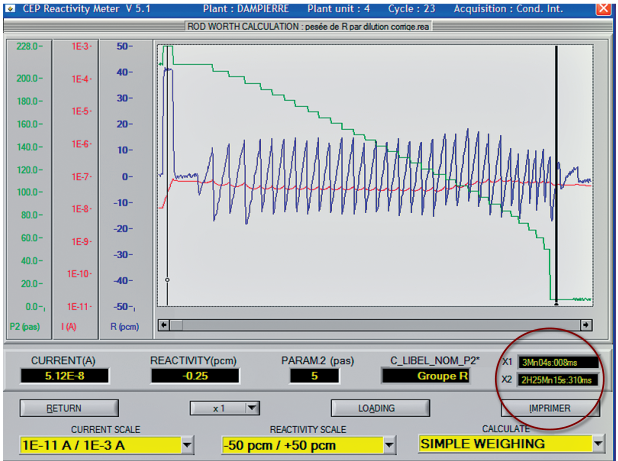
\includegraphics[width=4in]{images/pke/inhour-app.png}
  \caption{HZP Rod Worth Measurement: Boron Dilution}\label{inhour-app}
\end{figure}


%%%%%%%%%%%%%%%%%%%%%%%%%%%%%%%%%%%%% Inverse Kinetics %%%%%%%%%%%%%%%%%%%%%%%
\clearpage
\topic{Derivation of IK}
Assume we know the amplitude function $T(t)$ (that is, we are given a desired reactor power shape vs. time), we can solve for the precursor function $C(t)$; then plugging back in the PKEs, we can get $\rho(t)$, that is, how to operator reactor to achieve the desired power shape. 
\begin{enumerate}
\item Given $T(t)$, we can solve for the precursor equations, 
\begin{align}
\ddt C_i(t) &= \frac{\beta_i}{\Lambda} T(t) - \lambda_i C(t) \\
\ddt C_i (t) + \lambda_i C_i(t) &= \frac{\beta_i}{\Lambda} T(t) 
\end{align}
If we define matrix $[A] = \mathrm{diag}[\lambda_i], [B] = \frac{\mathrm{diag}[\beta_i]}{\Lambda}, [Y(t)] = [B] T(t)$, then the above equation forms a matrix system for all $i$,
\eqn{ \ddt [C(t)] + [A] [C(t)] = [B] T(t) = [Y(t)] }

\item Multiply by IF $[e^{At}]$, 
\begin{align}
[e^{At}] \ddt[C(t)]  + [e^{At}][A] [C(t)] &= [e^{At}] [Y(t)] \\
\ddt \left( [e^{At}][C(t)]  \right) &=  [e^{At}] [Y(t)]
\end{align}

\item Integrating both side from $0$ to $t$, define $C_0 = C(t=0), Y_0 = Y(t=0)$,  
\eqn{ [e^{At}][C(t)] - [C_0] &=  [A]^{-1} \left( [e^{At}] [Y(t)] - [Y_0] \right)  }
\eqn{ \Aboxed{ [C(t)] &= [e^{-At}][C_0] + [e^{-At}] [A]^{-1} \left( [e^{At}][Y(t)] - [Y_0] \right) } }
where $[A] = \mathrm{diag}[\lambda_i], [Y(t)] = \frac{\mathrm{diag}[\beta_i]}{\Lambda} T(t)$.
That is, we can solve for the time-varying concentrations of precursors for any desired reactor power shape in time by applying this equation successively for discrete steps. 

\item From the PKEs, we can solve for the reactivity in terms of $C(t), T(t)$ by making finite-difference approximation for derivative term: 
\eqn{ \ddt T(t) &=  \frac{\rho(t) - \beta}{\Lambda} T(t) + \Sum_i \lambda_i C_i (t) + Q(t) }
\begin{align}
\Aboxed{\rho(t) &= \frac{\Lambda}{T(t)} \ddt T(t) + \beta - \frac{\Lambda}{T(t)} \Sum_i \lambda_i C_i(t) - \frac{\Lambda}{T(t)} Q(t) } \\
\Aboxed{ \rho_n &= \frac{\Lambda}{T_n} \frac{T_n - T_{n-1}}{t_n - t_{n-1}} + \beta - \frac{\Lambda}{T_n} \Sum_i \lambda_i C_{i,n} - \frac{\Lambda}{T_n} Q_n } 
\end{align}
\end{enumerate}


\clearpage
\topic{Applications of IK}
IK is what is being used in production now. 
\subtopic{PWR Boration/Dilution}
\begin{figure}[ht]
  \centering
  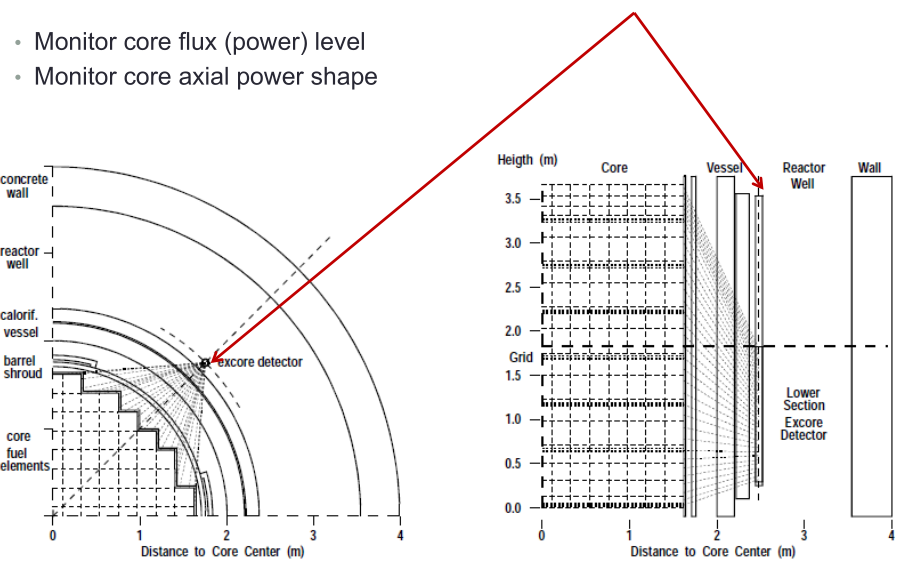
\includegraphics[width=4in]{images/pke/ik-ex1.png}
  \caption{IK Example 1, PWR Ex-core Detectors} \label{ik-ex1}
\end{figure}
The red lines in Fig.~\ref{ik-ex1} point out the location of the excore detectors. Prompt neutron life time is so short, so that even spatial distribution flux changes a lot, we can assume that it stabalizes already at each rod drop. 
\begin{itemize}
\item Disadvantages: time concern; boration dilution increases cost with waste disposal.  
\item Alternatives: we use General Inverse Kinetics to get around about it. 
\end{itemize}

\subtopic{SCRAM/Rod Drop Analysis}
  \begin{figure}[ht]
    \begin{subfigure}[b]{0.45\textwidth}
      \centering
      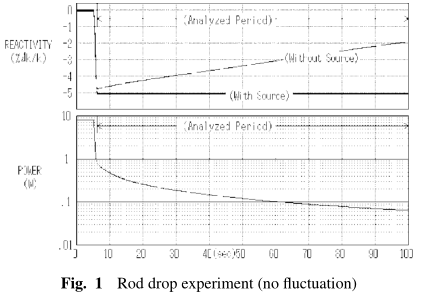
\includegraphics[width=\textwidth]{images/pke/ik-ex2a.png}      
      \caption{No Fluctuation} \label{ik-ex2a} 
    \end{subfigure}
    \begin{subfigure}[b]{0.45\textwidth}
      \centering
      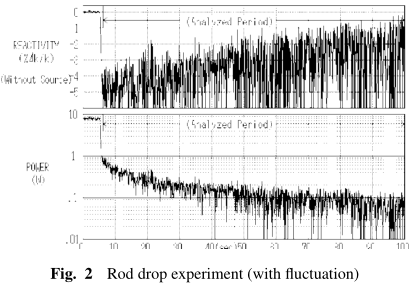
\includegraphics[width=\textwidth]{images/pke/ik-ex2b.png}      
      \caption{With Fluctuation} \label{ik-ex2b} 
    \end{subfigure}
    \caption{IK Example 2, Rod Drop for SCRAM Reactivity} \label{ik-ex2}
  \end{figure}
This example produces a scram, then measure power change and infer $T(t)$, thus estimate reactivity. The rough method use Prompt Jumpt Approximation. More accurately, we need to model all the neutron sources, including ($\alpha,n$) reactions etc. In reality, there are noisy signals in measured power and reactivity data; we need to smooth them out with a fitted function before we can apply IK with external neutron sources. The point is that we can use IK instead of prompt jump approximation to gain precision. 

This technique is not used in the US that much because it is harsh on your system and it requires work to bring the system back to critical. But it is one of the best ways to demonstrate to the licensing committee that a reactor is capable to scram.  

\subtopic{Dynamic Rod Worth}
This technique is widely used by Westinghouse to estimate their rod worth: starting with a critical reactor, and drive a control rod in and out and repeat with a different rod. 

The advantages are: no need to do boron dilution, and it takes 15 mins for each rod. 
\begin{figure}[ht]
  \centering
  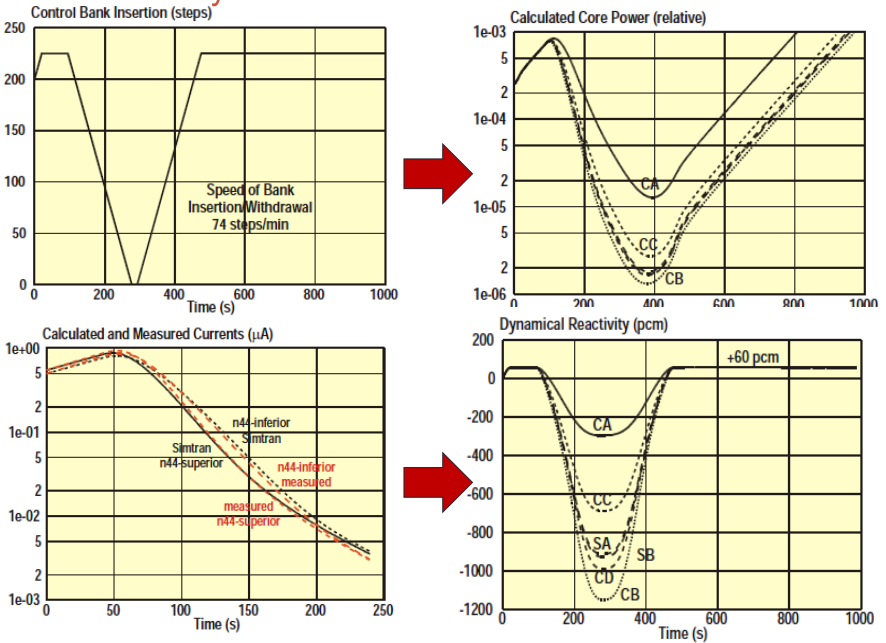
\includegraphics[width=4in]{images/pke/ik-ex3b.png}
  \caption{IK Example 3, PWR Dynamic Rod Worth} \label{ik-ex3}
\end{figure}

Alternatively, we can do sub-critical source multiplication, that is, IK with a source in the reactor. This way we don't even need to start with a critical reactor. This technique has only been used in experimental reactors but not so much in power reactors because it requires detailed knowledge about the source distribution. 

Note: we should be careful about power level. As shown in Fig.~\ref{power-range}, power can change from a few watts to 20,000 MW in less than a second! In order to make IK valid, we have to bring power down to make sure there is no thermal feedback. So it is a balance between getting a good signal and making sure there is no thermal feedback, thus people end up running the reactor in the intermediate range. 
\begin{figure}[ht]
  \centering
  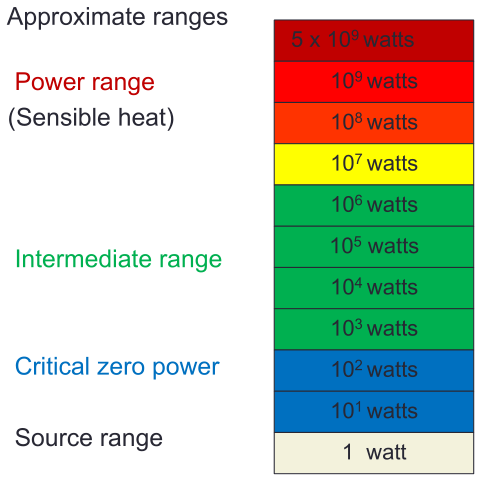
\includegraphics[width=4in]{images/pke/power-range.png}
  \caption{IK, Be Careful of Reactor Power Level} \label{power-range}
\end{figure}


\end{document}
